\section{Gráfico da Função Exponencial}
\begin{frame}
\frametitle{Gráfico da Função Exponencial} 

\begin{exemplo}
Seja $f: \R \to \R_+^\ast$ uma função exponencial tal que $f(x) =
a^x$. O gráfico de $f$ é:
\begin{center}
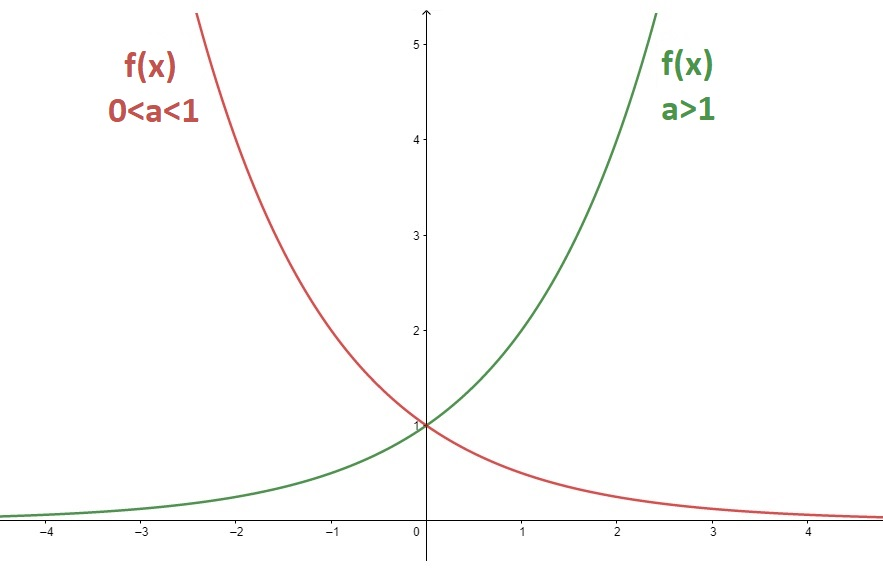
\includegraphics[width=6.3cm]{figures/grafexp.jpg}
\end{center}
O gráfico de $f$ nunca toca o eixo $x$, mas fica tão próximo quanto
queiramos. Isso equivale dizer que a reta $y=0$ é \sub{assíntota} do
gráfico de $f$.
\end{exemplo}

\end{frame}



%------------------------------------------------------------------------------------------------------------

\begin{frame}
\frametitle{Gráfico da Função Exponencial} 

\begin{exemplo}
O crescimento exponencial supera o de qualquer polinômio. Ao
compararmos, por exemplo, as funções $f(x) = 2^x$ e
$p(x)=x^{10}$, temos que:\\
\begin{tabular}{ccc}
$0<x<1{,}077$ & $\implica$ & $2^x > x^{10}$\\
$1{,}077 < x < 58{,}77$ & $\implica$ & $x^{10} > 2^x$\\
$x>58{,}77$ & $\implica $& $2^x > x^{10}$
\end{tabular}
\begin{center}
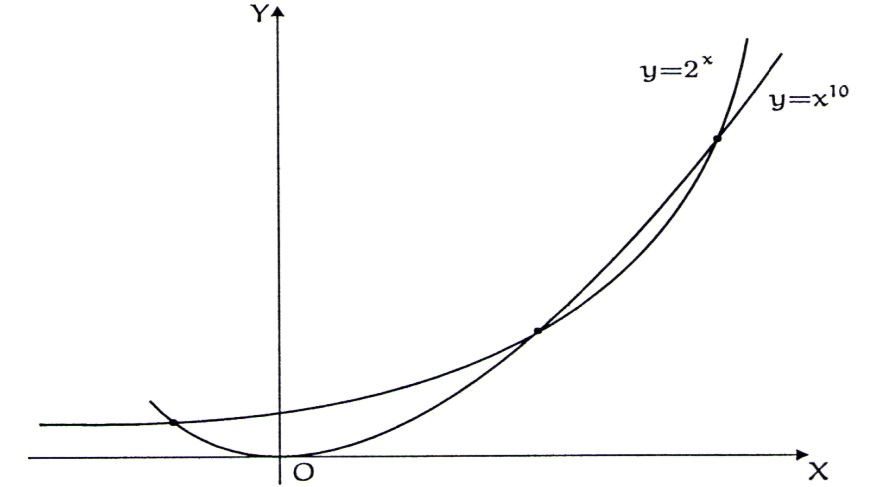
\includegraphics[width=7cm]{figures/polXexp.jpg}
\end{center}
\end{exemplo}

\end{frame}
